\chapter{Geological background}

To understand more about bank erosion, you must have knowledge about the soil profile of the delta region. This chapter intends to combine all the information found, regarding the soil, in our investigation area.

\section{The geology of a delta}


\section{Borehole}
One of the things that is found about the subsoil is a borehole. This borehole is done in the area of the port of Ibicuy. From this data is made the following soil profile \autocite{amatoESTRATIGRAFIACUATERNARIASUBSUELO2009};

\begin{figure}[H]
    \centering
    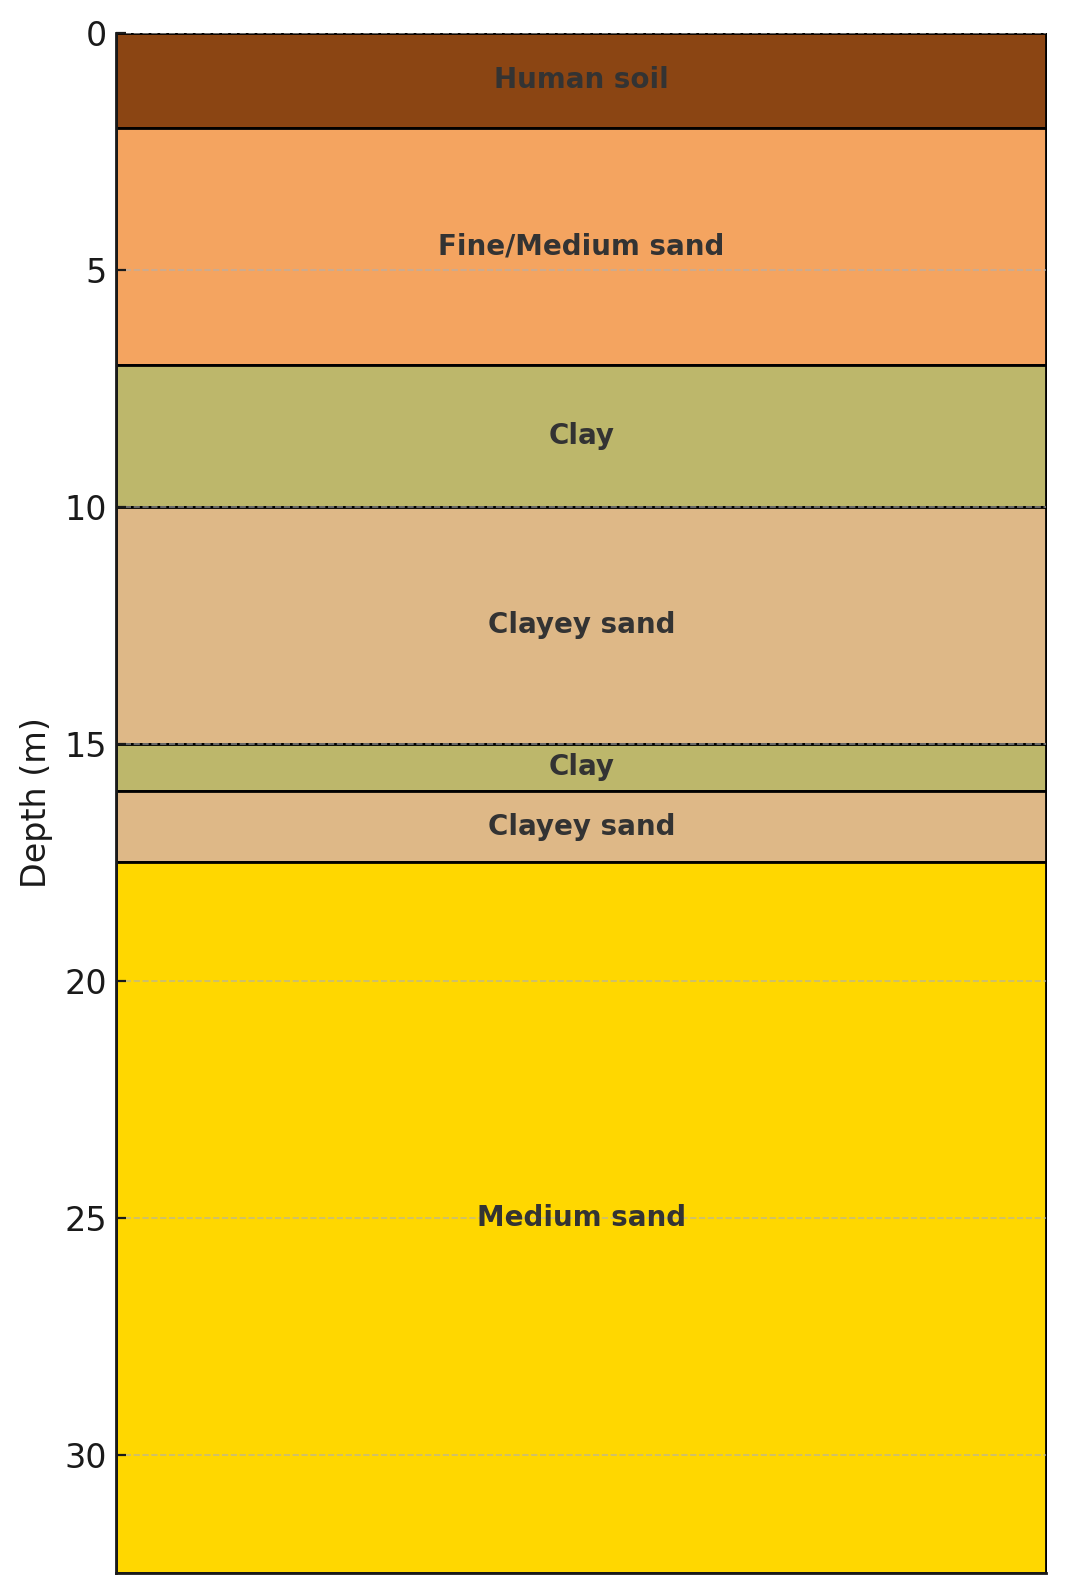
\includegraphics[width=0.45\linewidth]{figures//ch9/Bodemprofiel.png}
    \caption{Borehole profile}
    \label{fig:placeholder}
\end{figure}

\section{Geological cross section}
A study was conducted that led to a morphological map of the Paraná delta. In the study, for two cross sections a more detailed geological profile was made, one of which is relevant to the area of interest. The cross section along with the area is interest is shown in figure \ref{fig:crosssectiongeo}.

\begin{figure}
    \centering
    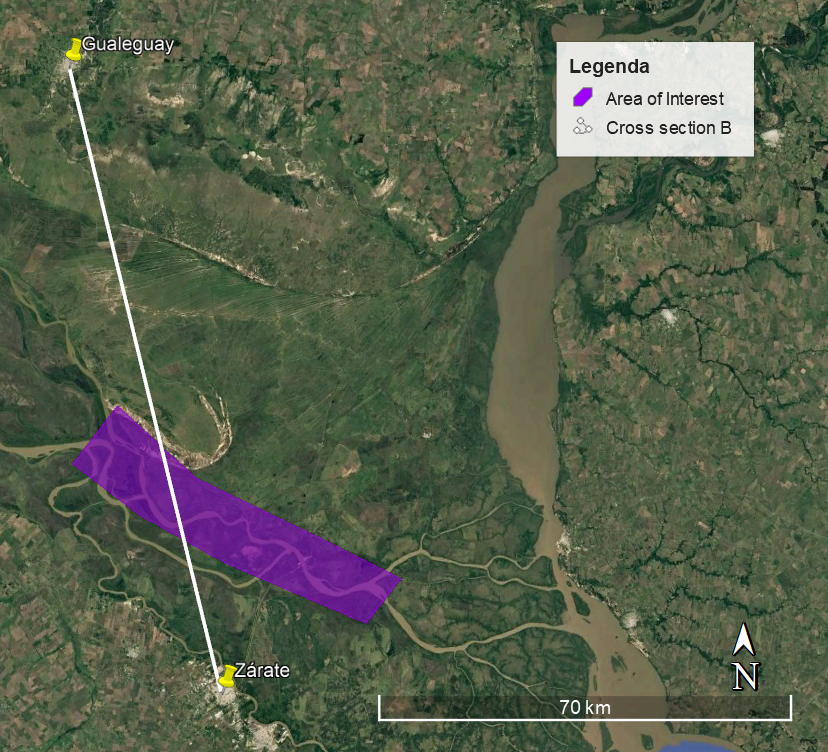
\includegraphics[width=0.75\linewidth]{figures/ch9/CrossSectionB.png}
    \caption{Cross section}
    \label{fig:crosssectiongeo}
\end{figure}

As can be seen in the figure, the taken cross section was around 